\documentclass[convert]{standalone}

\usepackage{tikz}
\usepackage{colortbl}
\renewcommand{\familydefault}{\sfdefault}

\begin{document}

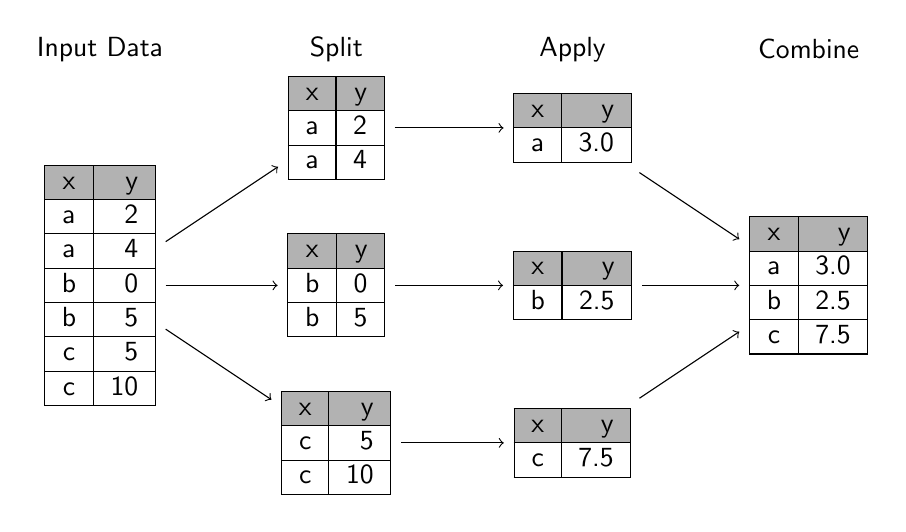
\begin{tikzpicture}

% Headings

\node (INPUT-LABEL)   at (0, 5) {Input Data};
\node (GROUP-LABEL)   at (3, 5) {Split};
\node (SUMMARY-LABEL) at (6, 5) {Apply};
\node (OUTPUT-LABEL)  at (9, 5) {Combine};


% Data Nodes

\node (INPUT)   at (0, 2) {

  \begin{tabular}{| c | r |}
    \hline
    \rowcolor[gray]{.7}
    x &  y \\ \hline
    a &  2 \\ \hline
    a &  4 \\ \hline
    b &  0 \\ \hline
    b &  5 \\ \hline
    c &  5 \\ \hline
    c & 10 \\ \hline
  \end{tabular}

};

\node (GROUP-A) at (3, 4) {

  \begin{tabular}{| c | r |}
    \hline
    \rowcolor[gray]{.7}
    x &  y \\ \hline
    a &  2 \\ \hline
    a &  4 \\ \hline
  \end{tabular}

};

\node (GROUP-B) at (3, 2) {

  \begin{tabular}{| c | r |}
    \hline
    \rowcolor[gray]{.7}
    x &  y \\ \hline
    b &  0 \\ \hline
    b &  5 \\ \hline
  \end{tabular}

};

\node (GROUP-C) at (3, 0) {

  \begin{tabular}{| c | r |}
    \hline
    \rowcolor[gray]{.7}
    x &  y \\ \hline
    c &  5 \\ \hline
    c & 10 \\ \hline
  \end{tabular}

};

\node (SUMMARY-A) at (6, 4) {

  \begin{tabular}{| c | r |}
    \hline
    \rowcolor[gray]{.7}
    x &    y \\ \hline
    a &  3.0 \\ \hline
  \end{tabular}

};

\node (SUMMARY-B) at (6, 2) {

  \begin{tabular}{| c | r |}
    \hline
    \rowcolor[gray]{.7}
    x &    y \\ \hline
    b &  2.5 \\ \hline
  \end{tabular}

};

\node (SUMMARY-C) at (6, 0) {

  \begin{tabular}{| c | r |}
    \hline
    \rowcolor[gray]{.7}
    x &    y \\ \hline
    c &  7.5 \\ \hline
  \end{tabular}

};

\node (OUPUT)   at (9, 2) {

  \begin{tabular}{| c | r |}
    \hline
    \rowcolor[gray]{.7}
    x &    y \\ \hline
    a &  3.0 \\ \hline
    b &  2.5 \\ \hline
    c &  7.5 \\ \hline
  \end{tabular}

};


% Arrows

\draw[->, to path={-> (\tikztotarget)}]
    (INPUT) edge (GROUP-A)  
    (INPUT) edge (GROUP-B)  
    (INPUT) edge (GROUP-C)

    (GROUP-A) edge (SUMMARY-A) 
    (GROUP-B) edge (SUMMARY-B) 
    (GROUP-C) edge (SUMMARY-C)

    (SUMMARY-A) edge (OUPUT)    
    (SUMMARY-B) edge (OUPUT)    
    (SUMMARY-C) edge (OUPUT)
;

\end{tikzpicture}

\end{document}

%------------------------
% References
% https://tex.stackexchange.com/questions/251642/draw-arrows-between-nodes-with-tikz
% https://tex.stackexchange.com/questions/11866/compile-a-latex-document-into-a-png-image-thats-as-short-as-possible
